% Small Models, Certified Behavior — draft 0.1 (paper-agent s-a1866810)
% Build: tectonic agent.tex   (bibtex-free; references are inline, as the language paper's)
\documentclass[11pt]{article}

\usepackage[a4paper,margin=1.1in]{geometry}
\usepackage{amsmath,amssymb}
\usepackage{microtype}
\usepackage{booktabs}
\usepackage{array}
\usepackage{enumitem}
\usepackage{xcolor}
\usepackage{tikz}
\usetikzlibrary{positioning,arrows.meta,fit,calc}
\definecolor{linkblue}{rgb}{0.1,0.15,0.45}
\usepackage[colorlinks=true,linkcolor=linkblue,citecolor=linkblue,urlcolor=linkblue]{hyperref}
\usepackage{cmap}
\emergencystretch=3em

% ---- notation (the language paper's) ---------------------------------------
\newcommand{\llp}{\textsc{llp}}
\newcommand{\metisc}{\texttt{metisc}}
\newcommand{\metispy}{\texttt{metispy}}
\newcommand{\agent}{\texttt{metis-agent}}
\newcommand{\lolli}{\multimap}
\newcommand{\orgurl}{\url{https://github.com/metis-lang-dev}}
\newcommand{\agenturl}{\url{https://github.com/metis-lang-dev/metis-agent}}
% a source pointer: the document section (and commit) a number comes from
\newcommand{\src}[1]{{\footnotesize\textsf{[#1]}}}

\title{\textbf{Small Models, Certified Behavior}\\[1ex]
\large A runtime that lends domain knowledge to local LLMs on robots and appliances}
\author{The metis project\thanks{Sources, the experiments' results, the fixtures and the
runtime: \agenturl{} and its sibling repositories at \orgurl. Correspondence:
\texttt{info@robofortis.com}.}}
\date{Draft 0.1 --- 2026-10-19}

\begin{document}
\maketitle

\begingroup\small\noindent
\textbf{How to read the numbers.} Every figure in this paper is taken from a
committed document, result file or test of the \agent{} repository or its
siblings, and is followed by a pointer \src{document \S\,section; commit}
to where it stands. Nothing was re-run for the paper. The experiments are the
record of a design being fixed by measurement, so some of them report a
configuration that was then rejected; the ruling that followed each one is
stated with it. The two sibling papers are \emph{Behavior Programs as Measures
over Proofs} (the language, draft 0.3) and \emph{Behavior Catalogs in
Practice} (the catalog and the loop, in preparation).
\endgroup

\begin{abstract}
A small local language model --- Gemma 4 E2B, 2.1\,GB resident on a laptop
GPU, or a CPU --- cannot be trusted to hold a device's procedure, state or
safety. We do not ask it to. \agent{} puts a \emph{certified runtime} in
charge: a behavior program from the catalog, in the language \llp{}, evaluated
exactly in about ten milliseconds, owning state, procedure, probability and
legality. The model gets narrow, checked jobs: map an utterance to one typed
intent, narrate what happened, propose an explanation for a surprise, ask the
person. Two agents share one kernel --- a \emph{domain agent} per loaded domain
(a mapper, a replier, a narrator, the runtime, a host) and an
\emph{orchestrator} per device (the dialog, routing, the floor) --- and the
device gets smarter by catalog changes through a human-gated loop, never by
retraining. We report the experiments that fixed the design: the model switch
(E2B maps the 54-turn dog corpus 54/54 at 458\,ms median, in 2136\,MiB); intent
as JSON text against native tool calls (E9: equal accuracy, the grammar
sampler costing at least 240 of J's 418\,ms mean); the executive's IO round-trip
(E10: the tool-response turn invites completion claims, so outcomes stay
text); the consult loop (E11: the harness owns the branch, the model chooses
within it); one model for both agents (NO-GO as a task, then measured: the same
reads at 1.4\,GB less, the sampled wording drifting past the model's 512-token
window); the specialist's limit (S1: a small model cannot continue a REPL read);
parity between the Python development stack and the Go embedded runtime on
recorded days (30 of 30 fixtures byte-equal, the C ABI's goldens 46/46, 95/95
and 43/43); and a CI job that runs the dog's turns on E2B on a public runner's
CPU in five minutes. We argue that the catalog's language --- atoms, intents,
replies and the rules' own \texttt{\%\%} lines --- is the emerging user
interface: what the person says, what the device says back and what a developer
edits are the same words.
\end{abstract}

\section{Introduction}\label{sec:intro}

Robots and appliances run offline, on small hardware, for years. A language
model is the natural front for them --- people speak, the thing answers --- and
a small one now fits: Gemma~4 E2B, quantized to four bits, is 2136\,MiB of
GPU memory on a laptop part \src{MODEL-EXPERIMENTS \S1, table 1} and runs on
four CPU cores at 17.9 tokens per second \src{catalog-packages step 1 B report;
\texttt{.github/workflows/model.yml}}. What a small model cannot do is own the
device. It forgets across turns, invents causes when none is given, reads an
acknowledgement as completion, and repeats a refused call. Every one of these
is measured below. None of them is a reason to use a bigger model; each is a
reason to give the model less authority.

The division this paper describes is one of \emph{authority, not speed}
\src{DESIGN ``Vocabulary''}. The certified side is a \llp{} behavior program:
a catalog of typed, staged, weighted linear-logic rules which denotes a
probability measure over its own runs (the language paper). Its runtime owns
state, procedure, probability and safety; every behavior is admitted through
gates; an evaluation costs about ten milliseconds; it is always on and never
waits for the model. The proposing side is the model: it narrates, maps a
request to one typed intent, proposes an explanation for a surprise, describes
an escalation. It is fallible by assumption, checked before every effect, and
its authority is revocable to zero --- the runtime's observe-only mode depends
on nothing the model says.

The paper sits in the middle of a three-layer stack. Below it is the language
and its toolchain (the OCaml compiler \metisc{}, the Python referee \metispy{},
a header-only C++ runtime, parity gates between them). Beside it is the catalog
--- a program as a package: one directory, one manifest, one loader --- and the
human-gated loop that grows a package by diffs a person approves (the catalog
paper). This paper is about what runs on the device: the agents, their
interfaces, the deployment shape, and the experiments that chose them.

\section{Architecture: two agents, one kernel}\label{sec:arch}

The design is stated for two agents on two models; running both on one small
model is an optimization, measured in \S\ref{sec:onemodel}, that changes none
of the interfaces \src{DESIGN v3 ``Architecture''}.

\begin{figure}[t]
\centering
\resizebox{\linewidth}{!}{%
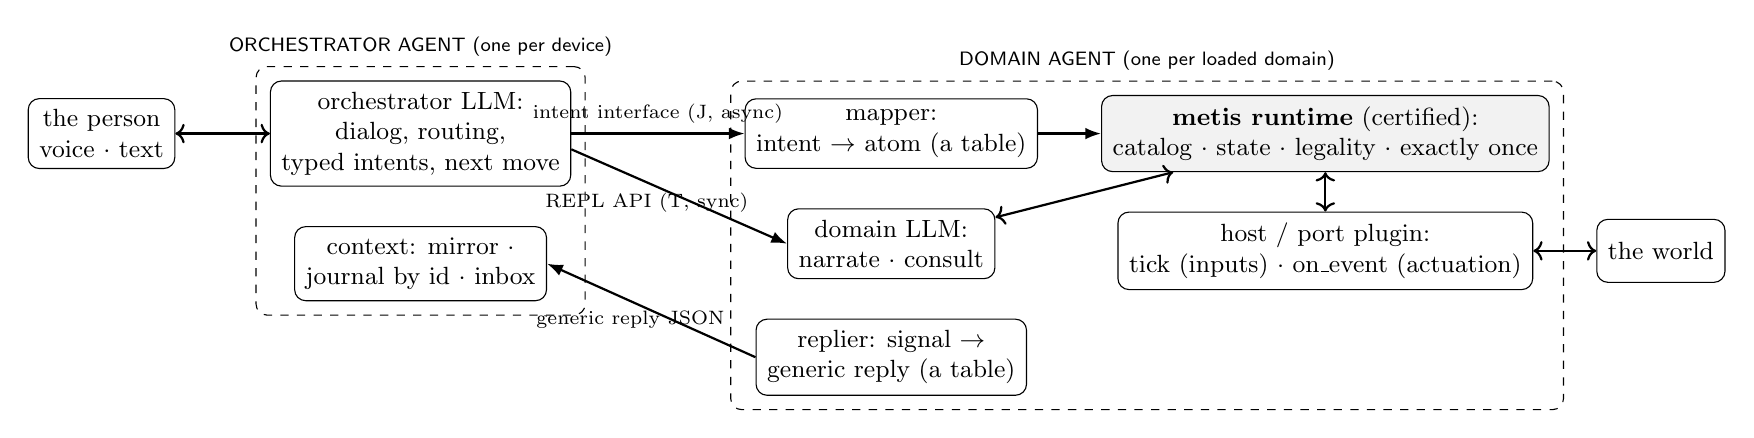
\begin{tikzpicture}[
  node distance=5mm and 7mm, font=\small,
  box/.style={draw, rounded corners, align=center, inner sep=4pt, minimum height=8mm},
  grp/.style={draw, dashed, rounded corners, inner sep=5pt},
  arr/.style={-{Latex[length=2mm]}, thick}]
  \node[box] (P) {the person\\voice $\cdot$ text};
  \node[box, right=12mm of P] (OL) {orchestrator LLM:\\dialog, routing,\\typed intents, next move};
  \node[box, below=of OL] (OC) {context: mirror $\cdot$\\journal by id $\cdot$ inbox};
  \node[grp, fit=(OL)(OC), label={[font=\scriptsize\sffamily]above:ORCHESTRATOR AGENT (one per device)}] (O) {};
  \node[box, right=22mm of OL] (DM) {mapper:\\intent $\to$ atom (a table)};
  \node[box, below=of DM] (DL) {domain LLM:\\narrate $\cdot$ consult};
  \node[box, below=of DL] (DR) {replier: signal $\to$\\generic reply (a table)};
  \node[box, right=8mm of DM, fill=black!5] (RT) {\textbf{metis runtime} (certified):\\catalog $\cdot$ state $\cdot$ legality $\cdot$ exactly once};
  \node[box, below=of RT] (HP) {host / port plugin:\\tick (inputs) $\cdot$ on\_event (actuation)};
  \node[grp, fit=(DM)(DL)(DR)(RT)(HP), label={[font=\scriptsize\sffamily]above:DOMAIN AGENT (one per loaded domain)}] (D) {};
  \node[box, right=8mm of HP] (W) {the world};
  \draw[arr, <->] (P) -- (OL);
  \draw[arr] (OL) -- node[above, font=\scriptsize]{intent interface (J, async)} (DM);
  \draw[arr] (OL.east) ++(0,-2mm) -- node[below, font=\scriptsize, pos=0.35]{REPL API (T, sync)} (DL.west);
  \draw[arr] (DR.west) -- node[below, font=\scriptsize, pos=0.6]{generic reply JSON} (OC.east);
  \draw[arr] (DM) -- (RT);
  \draw[arr, <->] (DL) -- (RT);
  \draw[arr, <->] (RT) -- (HP);
  \draw[arr, <->] (HP) -- (W);
\end{tikzpicture}}
\caption{Two agents and one kernel \src{DESIGN v3, the flowchart}. The runtime inside every
domain agent is the same certified interpreter; the orchestrator never touches it directly.
The line between the agents is who has to understand the domain: atoms, events, bindings and
ports are the domain agent's; the orchestrator knows a domain by its capability line, its
verb list and its mirror line.}
\label{fig:arch}
\end{figure}

\paragraph{Roles.} Table~\ref{tab:roles} is the design's own table of who owns what
\src{DESIGN v3 ``Roles''}. The model's column is short on purpose.

\begin{table}[t]
\centering\footnotesize
\begin{tabular}{@{}lll@{}}
\toprule
concern & owner & the LLM's part \\
\midrule
state over a long run & runtime & reads a mirror of it \\
step-by-step procedure & domain rules & picks which domain applies \\
uncertainty & runtime, exact inference & puts the result into words \\
safety and legality & orchestrator; observe-only on surprise & none; cannot override \\
when to think & orchestrator signals & wakes when signalled \\
changing the rules & revision loop, offline, human-approved & describes what went wrong \\
language and intent & orchestrator & one typed intent per request \\
understanding a domain & domain agent & narrates it; answers questions about it \\
judging a surprise & domain agent proposes, runtime checks & suggests which card explains it \\
the dialog with the person & orchestrator & speaks; asks; keeps the floor \\
\bottomrule
\end{tabular}
\caption{Roles \src{DESIGN v3}.}
\label{tab:roles}
\end{table}

\paragraph{The domain agent.} One per loaded domain, around one runtime serving one
catalog, on one host. Two of its five components are model work, three are tables and
code \src{DESIGN v3 ``The domain agent''}:
\begin{itemize}[nosep]
\item the \emph{narrator}: a runtime fragment $\to$ one sentence in the person's words,
  read against the catalog's \texttt{\%\%} comments (single pass, thinking off);
\item the \emph{consultant}: a question $\to$ a capped loop of REPL verbs $\to$ one typed
  answer (synchronous tool calls);
\item the \emph{mapper}: the intent JSON $\to$ one command atom from the card's table
  (\texttt{NAVIGATE goal=tag3} $\to$ \texttt{+cmd\_go(tag3)}); open-vocabulary targets
  resolve to the host's handles; quantities never enter the catalog --- they ride with the
  command in the host's queue and the port actuates with them; a verb with no row is an
  error. No model: a table, token-exact;
\item the \emph{replier}: a runtime signal or an intent's outcome $\to$ the generic reply,
  its \texttt{text} from the narrator. No model: a table over the wire's signals;
\item the \emph{host}: the port plugin, the catalog author's code: \texttt{tick} brings
  inputs as exogenous rows, \texttt{on\_event} actuates.
\end{itemize}

\paragraph{The orchestrator.} The person's counterpart and the manager of the domain
agents: it briefs, reads reports, decides the next move, asks the person when the world
lacks something. It never reasons about why a domain did what it did; it asks the domain
agent. Its context is laid out as regions ordered stable to volatile for the KV cache
\src{DESIGN v3 ``The orchestrator agent''}: a stable prefix (persona, the two interfaces,
the next-move table); a domains block (per loaded domain one capability line and its verb
list, never a nested schema); a journal (requests, intents by id and their outcomes,
consult answers, surprises); a mirror (one line per domain, overwritten in place); an
inbox (the one waking item).

\paragraph{Two interfaces out, no overlap.} Table~\ref{tab:ifaces} is the contract the
experiments of \S\ref{sec:exp} tested and amended.

\begin{table}[t]
\centering\small
\begin{tabular}{@{}>{\raggedright\arraybackslash}p{2.1cm}>{\raggedright\arraybackslash}p{6cm}>{\raggedright\arraybackslash}p{6cm}@{}}
\toprule
 & the intent interface & the REPL API \\
\midrule
shape & J: one JSON intent under the grammar built from the loaded verb lists & T: native tool calls, synchronous, one per turn \\
changes the world & yes: \texttt{call(domain, verb, args)}; the domain agent maps it to an atom, the runtime fires it under legality, the port actuates & no: it manages and reads \\
answered & later, by id: \texttt{accepted} now; \texttt{done} $\cdot$ \texttt{refused} (reason, alternatives) $\cdot$ \texttt{expired} $\cdot$ \texttt{progress} as they happen & now, in the tool response, and \emph{final}: \texttt{applied} $\cdot$ \texttt{admitted} $\cdot$ \texttt{refused} $\cdot$ \texttt{failed}; never \texttt{accepted} \\
verbs & the domain's dictionary (the dog: its eleven) & \texttt{activate}, \texttt{deactivate}; \texttt{state}, \texttt{ctx}, \texttt{events}, \texttt{why}, \texttt{findings}; \texttt{consult}; \texttt{reset}, \texttt{explain}, \texttt{escalate} \\
the person & --- & \texttt{ask(question)} is the orchestrator's own, as are \texttt{stop} and \texttt{cancel}, which fire on the keyword path before any model \\
\bottomrule
\end{tabular}
\caption{The orchestrator's two interfaces \src{DESIGN v3 ``Out, two interfaces''}. The
world is changed only through intents, which are linear and checked; everything synchronous
and read-only or administrative is the REPL API.}
\label{tab:ifaces}
\end{table}

\paragraph{The generic reply and the clock.} Every domain agent answers in one JSON shape:
\texttt{\{domain, kind, id, status, reason, alternatives, text, ref\}}, with \texttt{kind}
in result $\cdot$ event $\cdot$ quiescence $\cdot$ surprise $\cdot$ consult $\cdot$ ports;
the orchestrator's next move is a table over \texttt{kind} and \texttt{status}. Time is
beats: the host's tick at quiescence brings the world's inputs as one exogenous row, and
a beat may be \emph{scored} --- the runtime's likelihood of the host's reading given the
beat's start, and per action the program sent, the probability of the world's answer among
that action's alternatives (the catalog paper's measure).

\paragraph{The flow of one request.} The design's own example \src{DESIGN v3 ``The flow
of one request''}; \S\ref{sec:session} shows it as recorded:
\begin{quote}\footnotesize\ttfamily
person: "go to the kitchen"\\
orchestrator $\to$ intent \{"id":"c17","domain":"dog","verb":"NAVIGATE",\\
\phantom{orchestrator xxxxxxxxx}"args":\{"goal":"kitchen"\}\}\\
mapper \phantom{xxxx}$\to$ +cmd\_go(kitchen)\quad (the host's tick asserts it as an [env] row)\\
runtime \phantom{xxx}$\to$ go\_closed[P=kitchen] fires\\
\phantom{runtime xxxxxxx}(the only enabled rule: closed(kitchen) holds)\\
replier \phantom{xxx}$\to$ \{"kind":"result","id":"c17","status":"refused",\\
\phantom{replier xxxxxxx}"reason":"the way to it is closed", "text": ...\}\\
orchestrator $\to$ no alternatives $\to$ REPL consult(dog, "why is the way closed?")\\
consultant \phantom{x}$\to$ why refused(go) $\to$ closed(kitchen) $\to$\\
\phantom{consultant xxxxx}\{"answer\_kind":"missing", "resource":\{"atom":"closed(kitchen)",\\
\phantom{consultant xxxxxxxxxxx}"words":"the kitchen door"\}\}\\
orchestrator $\to$ ask(person, "The kitchen door is closed.\\
\phantom{orchestrator xxxxxxxxxxxxx}Should I wait, or go somewhere else?")
\end{quote}

\section{What the runtime gives the model}\label{sec:gives}

The model never sees the program. It sees what the runtime renders for it, and every
rendering is deterministic code, not a model's paraphrase --- a lesson E6 taught
(\S\ref{sec:e6}).

\paragraph{The mirror.} One line per loaded domain: stage, status, surprise state, the
declared beliefs (\texttt{\#query} marginals projected over the case horizon) and the
counts of the atoms the program names. Written by the harness from signals, overwritten
in place, at the head of each turn the harness writes \src{DESIGN v3; CML.md \S3}. It is
the runtime's state in the atoms' own names, \texttt{pred(args)}, and the orchestrator's
``what are you doing?'' is answered from it (E13 step 3, rule 4).

\paragraph{The journal by id.} Requests, intents with their ids and outcomes, consult
answers, surprises and how they ended; the model appends and compacts. The \texttt{dlg-*}
records of the journal are the same on both backends, so one reader
(\texttt{go/tools/live-reads.py}) scores either \src{DESIGN ``What parity means''}.

\paragraph{Surprise records and their triage.} The watch checkpoints the program at every
beat, reads the host, and prices the reading from the checkpoint. A reading no run reaches
is a surprise: the record carries the program key, the steps, the start, the observed
counts, the likelihood, its kind (\texttt{unmodeled} or \texttt{rare}) and the host's
snapshot as data, so it replays against the same world \src{metispy \texttt{kernel/record.py};
RUNTIME-PARITY row 17, 22}. On a surprise the domain goes observe-only; the model's part is
to propose a card and move that explain it, and the runtime checks the proposal as a witness
over the fired path. A surprise nobody explains is escalated to the people who revise the
model, with the record; it is not fixed on the device.

\paragraph{Intents, generated.} A domain's \texttt{intent.yaml} names the verbs, their
meanings, the persona and the examples; from it a generator writes the grammar
(\texttt{dog.gbnf}), the prompt, the spoken-response list and the corpus
(\texttt{intent/dog-corpus.tsv}, 54 rows). They are never written by hand \src{metis-catalog
\texttt{domains/dog/intent.yaml}; \texttt{tools/intents.py}}. The grammar pins the model's
turn to one JSON object the mapper's table admits: the certified surface stays token-exact.

\paragraph{The REPL tools, declared once.} The REPL's verbs are declared by \metispy{}
(\texttt{repl\_api}) and carried by every bundle as \texttt{tools.json}; both runtimes
render the same declarations, and the orchestrator's decider builds its own three from
that data \src{MODEL-EXPERIMENTS ``The decider's declarations'' (repl-tools step 3)}.

\section{Deployment shape}\label{sec:deploy}

\paragraph{Python develops, Go deploys.} \agent{}/\texttt{py} is the development stack:
the orchestrator and the domain agents run in one process, on one loaded model with three
contexts (orchestrator 16k, narrator 8k, consult seat 8k), with the console's backend in the
same process; the orchestrator's upper half and the domain agent's lower half are on separate
contexts on purpose, so an agent developing a domain can exercise the lower half with the
upper half emulated \src{DESIGN ``Two stacks, one behaviour''; agent-console step 2,
metis-agent 8d35cfa..3352be8}. \agent{}/\texttt{go} is the deployment runtime for the
embedded case: a small LLM with a text or voice interface on resource-constrained, offline
devices, the cost proportional to the intelligence required \src{RUNTIME-PARITY \S\,step 2}.

\paragraph{The runtime, bound.} The device runs the compiled program through a C ABI over
the language's header-only C++ runtime (\texttt{metis\_rt.h}, ABI~2, 23 exported symbols)
and a cgo binding (\texttt{go/internal/rt}): load the bundle's ground wire in the sidecar's
canonical order, bind the weight ports, seed, step, fire, enabled events, do-lines,
snapshot/restore, likelihood, hot reload with degrade-to-last-good. Through cgo the
language's goldens give IR parity 46/46, ground parity 95/95 and sample parity 43/43; live
parity against \metispy{}'s REPL on the dog (32/32 rows over 489 events), the plant with its
extension (30/30) and the kitchen pair (148/148 and 156/156, ports bound by Go), with
snapshot continuity and the recorded surprises' likelihoods equal at $10^{-12}$
\src{runtime-binding step 5 report; metis-lang 20096ed, metis-agent 3d99a75}. llama.cpp is
a submodule at a pinned commit, built once in CI and cached.

\paragraph{Parity on recorded days.} The generic domain agent exists twice --- Python over
\metispy{}, Go over the C ABI --- and the bar is logic parity: driven by the same inputs,
the same generic replies, the same records \src{DESIGN ``What parity means''}. Without a
model, the dog's, the plant's, the kitchen pair's and love\_triangle's scripted days are
dumped by Python and replayed into Go, the streams diffed as parsed JSON with likelihoods at
$10^{-9}$: 30 of 30 fixtures byte-equal, re-generated and compared on 2026-10-19
\src{\texttt{go/tools/dagent-parity.sh}; rddl-watch step 1 report}. With a model, the
orchestrator ported to Python decodes the same chunks under the same grammars and samplers as
the Go one (180/180 scenario replays, 42/42 timeline replays, mutation-checked), and on the
model 90 of 114 generations are identical, every first divergence at a token-equal context
and none moving a read; the remainder is the two llama.cpp builds' arithmetic, not the port
\src{agent-console step 2 report; DESIGN ``What parity means''}.

\paragraph{The adapter.} One finding is worth its line. The Python voice path was 12.89\,ms
per token against Go's 7.39 at 5.9k tokens of context, on the same library and the same
dialog; the cause was flash attention, which Go left at llama.cpp's default (on for this
model on CUDA) and Python had off. With it on, Python is 7.37\,ms per token and generates the
same greedy text; live, the service went from 18.4 to 9.5\,ms per token \src{llama-pin step
3 report; metis-agent 53ce367}.

\paragraph{The console.} The person meets the agent through a web page: fsttm-web's
dialog FSM (a finite-state turn-taking model keeps the floor; the models are senses and the
proposer, never the turn-taker), attention and speech, over one websocket protocol both
backends serve whole \src{DESIGN ``The process shape''; WIRE.md}. The agent console shows
every spoken line labelled by its source, the domains, each domain's REPL log, the world's
ports and the journal live.

\begin{table}[t]
\centering\small
\begin{tabular}{@{}>{\raggedright\arraybackslash}p{6.4cm}>{\raggedright\arraybackslash}p{3.9cm}>{\raggedleft\arraybackslash}p{4.4cm}@{}}
\toprule
what & where measured & number \\
\midrule
E2B Q4\_K\_M, text path, resident & M-E \S1, 8151\,MiB card & 2136\,MiB \\
E2B Q4 + whisper base.en, co-resident, one process & M-E budget line & 2368--2374\,MiB \\
Go service (E2B + the dog's prefix + the orchestrator 8k) & integration step 3 & 2868--2874\,MiB \\
py domain agents (dog, kitchen, kitchen\_shared) & integration step 3 & 2360--2370\,MiB \\
both resident & integration step 3 & 5339\,MiB (2.7\,GB free) \\
live service, two models $\to$ one model (the session's end) & go-domain-agent step 6 & 3846 $\to$ 2436\,MiB ($-1410$) \\
voice, ms per token at 5.9k context, py off $\to$ py AUTO $\to$ Go & llama-pin step 3 & 12.89 $\to$ 7.37 $\to$ 7.39 \\
voice, ms per token live & llama-pin step 3 & 18.4 $\to$ 9.5 \\
a person turn: move generation, median & integration step 3 (go-scripted) & 464\,ms \\
a spoken line: voice generation, median & integration step 3 & 68\,ms \\
a reply $\to$ its line spoken, median & integration step 3 & 80\,ms \\
the wire, per intent (a tool call waits for its answer: the kitchen's consult, 6.9\,s) & integration step 3 & 0--1\,ms \\
a beat with the narrator & integration step 1 run 2 & 113\,ms \\
CI, E2B on a public runner's CPU: 3 tests & model.yml, first run & 5\,min 14\,s \\
llama-bench pp512 / tg64, 4 threads, CI's CPU build (local) & catalog-packages 1B & 123 / 17.9 tok/s \\
\bottomrule
\end{tabular}
\caption{Deployment numbers. M-E is MODEL-EXPERIMENTS.md; the step reports are the subjects'
committed reports.}
\label{tab:deploy}
\end{table}

\section{Experiments that fixed the design}\label{sec:exp}

Each experiment was pre-registered with its reads and a decision rule, run by one
implementer, and ruled by the architect. They are held in one document,
\texttt{docs/MODEL-EXPERIMENTS.md}, and the numbers below are its, verbatim.
Table~\ref{tab:outcomes} is the summary.

\subsection{The model switch (E1--E3)}\label{sec:e1}

The question was whether Gemma~4 E2B or E4B could replace gemma3:4b as the intent model,
within an 8\,GB GPU budget shared with ASR. Same harness, same 54-turn dog corpus (34 prompt
rows, 20 held-out), same adapter \src{M-E \S1, table 1; results/e1-p2ex}.

\begin{table}[h]
\centering\small
\begin{tabular}{@{}lrrrrr@{}}
\toprule
model & VRAM & turn p50 / p90 & intent & held-out & narrate leak \\
\midrule
gemma3-4b Q4 (before) & 3556\,MiB & 506 / 833\,ms & 52/54 & 16/17 & 44/54 \\
\textbf{E2B Q4} & \textbf{2136\,MiB} & \textbf{458 / 722\,ms} & \textbf{54/54} & \textbf{17/17} & 0/54 \\
E2B Q5 & 2374\,MiB & 466 / 742\,ms & 54/54 & 17/17 & 0/54 \\
E4B Q4 & 3810\,MiB & 603 / 960\,ms & 52/54 & 15/17 & 0/54 \\
E4B Q5 & 4292\,MiB & 637 / 992\,ms & 53/54 & 16/17 & 0/54 \\
\bottomrule
\end{tabular}
\caption{E1, the intent model on the text path \src{M-E \S1}. ``Narrate leak'' is the bare
single-pass path, not the harness's; through the harness both models narrate cleanly.}
\label{tab:e1}
\end{table}

The ruling: E2B Q4\_K\_M, thinking off \src{M-E ``Results and recommendation'';
metis-agent 875c219}. E4B bought nothing and cost about 2\,GB; thinking bought nothing on
intent and 1.3--1.6\,s per turn. On narration of 24 failed or refused outcomes, both models
pass the guard 24/24, but they differ in fidelity: gemma3 invents causes when none is
given (``because my joints are stiff''); E2B states the given reason, formulaically, at
108\,ms median against 165 \src{M-E \S2}. For ASR, whisper base.en with a command-vocabulary
initial prompt gives 1.9\% WER on the rendered corpus and 53/54 intents after transcription,
in 409\,MiB; the streaming Nemotron candidate gave 9.6\% and does not endpoint by itself
\src{M-E \S3, E2}. The heard path (Gemma~4's native audio into the same grammar) matches
the pipeline on accuracy and latency but costs about 0.8\,GB more and leaves no transcript,
so it is not recommended yet \src{M-E \S4, E3}.

\subsection{E6: does a spliced fact steer the continuation?}\label{sec:e6}

Under the stream idea (CML.md): a runtime result formed into a short text piece and
inserted into an ongoing context --- does the model reason from it? Twelve real runtime
facts from the kitchen fixtures, three renderers, three insertion forms, three distances
\src{M-E E6/E6b; results/e6}. The finding: inline at distance zero, yes, with plain words
--- the plain-word template T2 reaches 0.92 (thinking off) and 1.00 (thinking on), while
the model's own zero-context narration of the raw line loses everywhere (0.25--0.42). A
fact does not carry across turns reliably (0.42--0.75 at six turns), the newer of two
values does not win reliably (0.75 newer / 0.08 older), and a third of all answers open by
copying the spliced line back; up to 0.19 of answers under some forms \emph{forge} a
fragment in the runtime's syntax with a fact the runtime never sent. The rulings: the
renderer stays deterministic; standing facts go in the mirror, overwritten in place;
compaction deletes a superseded fact; and a model output carrying the fragment syntax is
refused, never spoken \src{M-E E6 ``What this says''; metis-agent 9eba55d}.

\subsection{E9: native tool calls against the JSON two-pass}\label{sec:e9}

Gemma~4 is trained for function calling; the harness maps an utterance to JSON under a
grammar, then continues with a bare ``Spoken response:'' cue. Does the native call beat
the JSON on the corpus we have, and what does the grammar cost? Five arms on E2B
\src{M-E E9 findings; results/e9}.

\begin{center}\small
\begin{tabular}{@{}lrrrr@{}}
\toprule
arm & class & JSON identical & ms to intent p50 & prefix tokens \\
\midrule
J (the JSON two-pass, control) & 54/54 & 54/54 & 416 & 1491 \\
J-free (no grammar) & 54/54 & 54/54 & 175 & 1491 \\
T (native call, grammar-pinned) & 54/54 & 52/54 & 531 & 3481 \\
T-free (native call, unpinned) & 53/54 & 52/54 & 154 & 3481 \\
T-noex (no examples) & 50/54 & 32/54 & 493 & 2461 \\
\bottomrule
\end{tabular}
\end{center}

Class ties, 54/54; the tool call loses two rows on arguments and is 112\,ms slower from
its larger grammar; without the 40 examples both class and arguments fall. The ruling: J
stays \src{M-E E9 ruling}. The finding to act on is latency, not format: the grammar
sampler costs at least 240 of J's 418\,ms mean (p50 416), and unpinned the model writes a well-formed,
correct JSON on 54/54 rows in at most 178\,ms --- free-then-verify (E9b) is the proposal
that acts on it. The certified surface stays grammar-pinned because nothing unvalidated may
reach the dispatcher; these numbers are the price of that.

\subsection{E10: the executive's IO round-trip}\label{sec:e10}

E9 compared classifiers. E10 tested the formats as an \emph{API}: typed calls down,
responses the model consumes up, sync and async on the same turn type, over a synthetic
corpus of 282 scripted dialogs with injected responses and signals, scored by rules
\src{M-E E10 run; results/e10}. The tool-call arm failed the parity bar (class 52/54, 3
leaks, 4 completion claims against \texttt{accepted}) and won none of the deciding groups;
it won only interleaving (9/10 against 4/10) because its response carried the call's id.
The ruling: JSON text stays in both directions \src{M-E E10 ruling, user confirmed}. What
the three tool-call experiments taught together: accuracy does not depend on the format
(the rows a small model gets right are decided by the examples it is shown); declarations
cost context the small model pays for (5.2k against 2.8k prefix tokens, two held-out rows);
the response turn carries a trained prior --- \emph{call, result, done} --- so every arm
that saw a result turn reported a task complete on some acceptances and the JSON path
never did; and identity in the outcome, not the format, prevents cross-wiring. E10b showed
the hand-rendered declarations are the GGUF template's rendering byte for byte (17 of 17),
and that E4B does not close the gap \src{M-E E10b ruling}.

\subsection{E11: the consult loop}\label{sec:e11}

After a refusal or a failure, does E2B make the right next move: call an offered
alternative, consult, explain, ask, reset or escalate, and never repeat the refused call?
Sixty-six items in five groups, reads pre-registered \src{M-E E11; s-a0477202}. Run 1, with
a generic cue, failed three of four reads: the model consults when alternatives are offered,
escalates when it should consult, repeats a consult when the same refusal returns. Run 2
changed the harness, not the prompt: the cue names the branch the harness already knows
(alternatives offered $\cdot$ none $\cdot$ a consult answered $\cdot$ the same refusal
again), the next-move grammar is restricted to that branch's moves, the explanation line is
templated. Then G1 12/12, G2 11/12, G3 23/24, G4 6/6, the ask on every missing-resource
item and nowhere else, 0 repeats, 0 leaks and claims over 66 lines. Adopted \src{M-E E11
ruling}. What the two runs settled is the division of labour this paper is about: the
harness owns the branch; the model chooses within it and speaks.

\subsection{E13 and integration: the dialog under control}\label{sec:e13}

E13 moved the pieces into the Go orchestrator and measured it against emulated domains ---
the dog with live tasks, the kitchen sending orders and signals unasked --- on 14 timelines
$\times$ 3 seeds with bars on ids kept straight, the floor honoured, the person's answer
bound to its question, zero signals read as commands, speech clean \src{M-E E13 steps
1--3}. Three runs and three rulings later every read held: an outcome's line names its own
task 45/45, the opener's domain and record carried 24/24, no generation on an event or a
notice, yes $\to$ the retry 12/12, no $\to$ no world-changing intent 3/3, a new command
closes an open question 3/3, every intent allowed 78/78, 0 leaks, 0 claims, 0 ids aloud
\src{M-E E13 step 3 run 3b ruling}. Nine harness rules came out of it, all in the design:
the bound answer is classified, not moved; the intent pass runs first on a bound turn; the
offered verb on a busy question is yes; the outcome turn leads with the task's words; the
ask check takes the resource's key; an information turn speaks from the mirror; no intent
speaks at the person's turn --- the first reply speaks. The real dog behind the orchestrator
then held the same bars (R1a 45/45, R4 78/78) after five more rules the real world exposed
\src{M-E Integration step 1 run 2 ruling; s-f82a578f}. Two further rulings from the live
measure: the orchestrator's dialog room went to 16k tokens (+106\,MiB), and the surprise's
consult runs off the orchestrator's turn so a person is never queued behind it --- a dog
command typed one second into a 7.5\,s consult is dispatched in 596--687\,ms and its first
line spoken within the beat \src{integration step 3; agent-console step 2 \S5}. Time and
date answer from the clock, never from the model.

\subsection{E12: one model for both agents}\label{sec:onemodel}

The integration measure ruled the single-model optimization \textbf{NO-GO as a task}: two
E2B instances take 5.3 of 8.1\,GB and VRAM does not bind; one model would serialize the
kitchen consult (6.9\,s) with the orchestrator's own generations; and the one-process shape
makes weight-sharing nearly free later \src{integration step 3 ``E12''}. It was then built
as the Go deployment's shape and measured on the same reads \src{go-domain-agent step 6;
metis-agent 60ccbe0, 7074f98}: the orchestrator and every narrator are roles on one loaded
context, each with its own budget, prefix, tape and sampling, swapped by KV state
save/load (204 swaps in a 14-timeline replay, about 24\,ms each). Every read is identical
to the two-model run; the dispatched intents are equal 7/7 live; the live service's VRAM
falls from 3846 to 2436\,MiB at the session's end ($-1410$; 3792 to 2432 at its start). One finding, with its cause established: past Gemma~4's 512-token
sliding window a restored KV is exact in content but laid out differently, the attention's
fp16 accumulation moves, and a \emph{sampled} line can take another word --- greedy moves
keep their argmax, so no read and no dispatch moves. Byte-exact one-model would need a
layout-preserving restore; it is a follow-up, not a blocker.

\subsection{S1: the specialist's limit}\label{sec:s1}

Can a small model be the kernel's user --- continue a REPL read, call \texttt{why},
\texttt{necessity}, \texttt{sufficiency} on what it sees and answer faithfully? Twenty
items, two reads (reached, faithful), four Gemma seats and Claude as the baseline
\src{SPECIALIST \S5b; metis-agent 94cbaea, df1db14}. Reached / faithful of 20: E2B off 10 /
1; E2B with a 256-token thinking cap 16 / 6; E4B off 16 / 8; E4B cap 19 / 7; Claude 20 /
15 (18 by hand). Read 1 holds for E2B with the cap and for E4B; read 2 fails on every Gemma
seat, and necessity is where the small model is furthest behind on every seat (Claude 5/5,
Gemma $\le$ 2). Under the pre-registered rule the specialist line does not continue on the
small model as it stands. About half the misses were an argument the kernel could not hold
--- \texttt{state} printed atoms grouped by predicate while the instruments take
\texttt{pred(args)}, a form no output the model saw ever printed --- which is the class of
error every E-series found and fixed on the harness side; S1b re-registered that one form
change (\metispy{} 11c9236) and the bars stand. The consultant stays in the domain agent for
the restricted, measured use it has: a surprise with cards, kinds and moves pinned, where the
kind is computed from the host's complementary pairs and not chosen by the model at all
\src{DESIGN v3 ``The domain agent'', system prompt part 2}.

\subsection{E7/E8: retrieval}\label{sec:rag}

Does structural retrieval over the runtime's fragments beat flat mixing of the last pieces
of each domain's tape? Run 2: attribution S 0.80 = F 0.80, tokens S 246 $<$ F 254, invented
0 everywhere; the display names, not the retriever, are what made the model attribute a
fact to its domain (three questions went 0/3 $\to$ 3/3 in every arm) \src{RAG \S10,
metispy bf52dbd}. The read: flat mixing suffices until a tree exists; the RAG stays an
experiment. What stands in the harness: fragments tagged with the domain's display name in
the person's words, one tape per domain on one clock, cross-domain moves naming their
target. Triage (which card explains a surprise) was measured apart: the arms without the
tape did as well as with it (B 1.00, C 1.00 against A 0.60), so the tape was dropped from
triage and the decider runs on the surprise and the cards alone.

\subsection{CI on a public runner}\label{sec:ci}

The model path --- the two-pass intent, the tape kept through turns, two roles on one
context --- had no CI at all: its tests skip without weights. A workflow of its own now
runs E2B Q4\_K\_M on CPU on a public runner: the weights pinned by revision and sha256,
public and ungated under Apache-2.0, cached; llama.cpp built once with CI's flags; three Go
tests on the dog's prompt and grammar, with a skipped load counted as a failure; daily, on
dispatch, and on a push that touches the adapter, the agent or the llama.cpp pin --- never a
required check \src{\texttt{.github/workflows/model.yml}; metis-agent 737c4ac, 896f1cb}.
Locally with CI's build on four cores: prompt evaluation 123 tokens/s, generation 17.9, one
dog verb turn 1.66\,s mean, the 54-row corpus 54/54; the first run on GitHub took 5\,min
14\,s and passed \src{catalog-packages step 1 B report}. The splice test is left out: on
CPU, a spliced KV and the same tape decoded at once part after about fifteen tokens --- a
numerics limit of an exact-equality test, not a regression, and the same arithmetic the
one-model finding of \S\ref{sec:onemodel} met.

\begin{table}[t]
\centering\small
\begin{tabular}{@{}>{\raggedright\arraybackslash}p{1.3cm}>{\raggedright\arraybackslash}p{4.4cm}>{\raggedright\arraybackslash}p{4.9cm}>{\raggedright\arraybackslash}p{3.7cm}@{}}
\toprule
 & what was asked & result & ruling \\
\midrule
E1--E3 & E2B/E4B as the proposer; ASR; heard vs read & E2B Q4: 54/54, 458\,ms, 2136\,MiB; whisper + prompt 1.9\% WER; heard = pipeline, +0.8\,GB & E2B Q4, thinking off, whisper \\
E6 & a spliced fact steers the continuation? & 0.92--1.00 inline at distance 0 in plain words; not across turns; forgeries & deterministic renderer; mirror for standing facts; fragment syntax refused \\
E9 & native tool call vs JSON two-pass & class tie 54/54; args 52 vs 54; +112\,ms; grammar $\ge$ 240\,ms & J stays; E9b proposed \\
E10 & tool call as the API & T fails parity (52/54, 3 leaks, 4 claims); wins only interleaving & J-text both ways; identity in the outcome \\
E11 & the consult loop & generic cue fails 3/4 reads; branch cue + restricted grammar: all hold & adopted: the harness owns the branch \\
E13 & dialog control vs emulated domains & every bar after 3 runs; 9 harness rules & phase 2 complete \\
integration & the real dog behind it & every bar after 5 more rules & phase 3 step 1 done \\
E12 & one model for both agents & NO-GO as a task; built later: reads equal, $-1410$\,MiB, sampled wording drifts & the Go deployment's shape \\
S1 & the model as the kernel's user & read 2 fails on every Gemma seat (E4B off 8/20; Claude 15) & the specialist waits for a stronger small model \\
E7/E8 & structural RAG vs flat mixing & S 0.80 = F 0.80; names did it & flat mixing; the RAG an experiment \\
\bottomrule
\end{tabular}
\caption{The experiments in one table \src{MODEL-EXPERIMENTS.md; SPECIALIST.md; RAG.md;
the integration and go-domain-agent reports}.}
\label{tab:outcomes}
\end{table}

\section{Language as the emerging user interface}\label{sec:language}

The same words appear three times, and that is the point.

\paragraph{What the person says.} The intents are a vocabulary the catalog declares:
eleven verbs for the dog, their meanings in a sentence each, the examples the grammar is
generated from, the persona --- ``You are Nina, a quadruped robot dog'' --- all in
\texttt{intent.yaml} \src{metis-catalog \texttt{domains/dog/intent.yaml}}. The grammar
over the intent schema is a UI contract: whatever is said, what reaches the device is one
object the table admits, and the 54-row corpus is the contract's test.

\paragraph{What the device says back.} Every rule carries a \texttt{\%\%} line in the
device's voice --- \texttt{\%\% I sit down.} above \texttt{sit [dyn] : cmd\_sit * posture(P)
* \ldots}, \texttt{\%\% I can't go to \{P\}: the way to it is closed.} above
\texttt{go\_closed} --- and the narrator fills the binding (\texttt{\{P\}} $\to$ ``the
kitchen'') from the host's display names. The generic replies are templated from the same
lines; the consult's resource words (``open the way to the kitchen'') are the host's table's,
not the model's, since E2B wrote usable words 1 time in 4 \src{DESIGN v3 ``Open, settled
2026-10-14''}. A refusal names its blocker in the words the person can act on.

\paragraph{What the developer edits.} The program, its \texttt{\%\%} lines, the intent file
and the extensions are the files the loop proposes as diffs and a person approves (the
catalog paper): the words the device will say are reviewed in the same gate as the rule
that makes it say them. A change of behaviour is a change of text, never of weights.

\paragraph{Honest limits.} The narration is formulaic (``My command to \ldots{} failed
because \ldots''); there are tautologies (``lost sight of you because I couldn't see you'');
an adversarial instruction planted in a detail field is repeated, not obeyed
\src{M-E \S2}. The runtime's own detail text is what gets repeated, which is a harness
concern; the remedy applied is the guard, which turns anything unspeakable into ``Okay.''.

\section{A session, as recorded}\label{sec:session}

Figure~\ref{fig:session} is the opening of the dog's recorded day, the fixture the Python
and Go domain agents are held equal on \src{\texttt{go/internal/dagent/testdata/days/dog.out.jsonl},
rows c1--c2}: an intent in, \texttt{accepted} now, the rule that fired a beat later with the
device's line, a refusal with its reason and alternatives, and the consult that turns the
refusal into what the person can do. Every line is the fixture's.

\begin{figure}[t]
\begin{quote}\footnotesize\ttfamily\raggedright
$\to$ \{"id": "c1", "domain": "dog", "verb": "LOCAL\_ACTION", "args": \{"action": "SIT\_DOWN"\}\}\\
$\leftarrow$ \{"kind": "result", "id": "c1", "status": "accepted", "text": "Accepted."\}\\
\quad beat 2, event sit[P=standing]\\
$\leftarrow$ \{"kind": "result", "id": "c1", "status": "done", "text": "I sit down.", "voice": "line"\}\\[1ex]
$\to$ \{"id": "c2", "domain": "dog", "verb": "NAVIGATE",\\
\quad\ "args": \{"goal": \{"type": "REGION", "description": "kitchen"\}\}\}\\
$\leftarrow$ \{"kind": "result", "id": "c2", "status": "accepted", "text": "Accepted."\}\\
\quad beat 4, event go\_closed[P=kitchen]\\
$\leftarrow$ \{"kind": "result", "id": "c2", "status": "refused", "reason": "the way to it is closed",\\
\quad\ "text": "I can't go to the kitchen: the way to it is closed.",\\
\quad\ "alternatives": [\{"verb": "go", "args": \{"place": "door"\}\},\\
\quad\quad\quad\quad\quad\quad\quad\quad\quad\ \{"verb": "go", "args": \{"place": "tag3"\}\}]\}\\[1ex]
$\to$ \{"tool": "consult", "args": \{"question": "why did you not go?"\}, "id": "k1"\}\\
$\leftarrow$ \{"kind": "consult", "id": "k1", "answer\_kind": "missing",\\
\quad\ "resource": \{"atom": "closed(kitchen)", "words": "open the way to the kitchen"\},\\
\quad\ "evidence": ["closed(kitchen) 1", "mapped(kitchen) 1"], "calls": 0\}
\end{quote}
\caption{The dog's recorded day, rows c1, c2 and k1 of \texttt{dog.out.jsonl} (fields
abridged; the person's words for these intents are the corpus rows ``sit'' and ``go to the
kitchen''). The consult's answer is computed, not generated: \texttt{missing} because the
host's pair \texttt{open|closed} can be flipped by the person, the words from the host's
table; \texttt{calls: 0} --- no model call was needed.}
\label{fig:session}
\end{figure}

\section{Related work}\label{sec:related}

The rules are in the Ceptre lineage of linear-logic programming for interactive worlds
(Martens, \emph{Ceptre: a language for modeling generative interactive systems}, AIIDE
2015); what metis adds is the measure over runs and the certified evaluation (the language
paper). Turn-taking is the finite-state turn-taking model of Raux and Eskenazi (NAACL-HLT
2009), kept as the dialog engine in front of every model. Constraining a model's output to
a grammar is llama.cpp's GBNF sampler; \S\ref{sec:e9} measures what it costs here. LLM
agents that act through
tools (the ReAct line, Yao et al., ICLR 2023) put the model in charge of the loop; here the
loop is the harness's and the model's authority is a table of narrow, checked jobs
(Table~\ref{tab:roles}). Neuro-symbolic planners pair a model with a planner it calls; here
the planner side is a probabilistic program whose every evaluation is exact and whose
surprise is a measured zero, and the model never calls code --- what it may ``call'' is a
catalog domain. On-device models: the budget line of Table~\ref{tab:deploy} is the whole of
our claim about size.

\section{Limits and what is next}\label{sec:limits}

Observe-only is the fallback, and it depends on nothing the model says: a device whose
model is wrong, slow or absent still runs its program, refuses what is illegal and records
what it cannot explain. The model's authority is revocable to zero by construction.

Not covered here: the user's real recordings (the ASR and heard-path decisions wait for
them \src{M-E ``Open items''}); the heard path's projector re-pack; a traffic simulator
runtime for the road domain; and the tuning of the RDDL worlds' programs against their gyms,
which the catalog paper's measure now makes possible and this design keeps off the device.
The specialist waits for a stronger small model, or a kernel-side form change that S1b
measures. Byte-exact one-model serving needs a layout-preserving KV restore. The orchestrator
has no journal compaction yet: near the context's end the dialog starts over, which E6 ruled
the safe version. Each of these is a subject with a pre-registered read, as everything above
was; the record is the repository.

\section*{Sources}

\begin{small}
\begin{tabular}{@{}p{3.6cm}p{11.2cm}@{}}
\toprule
pointer & document (and commit) \\
\midrule
DESIGN & \agent{} \texttt{docs/DESIGN.md} v3 (2026-10-13; the process shape 2026-10-14, two stacks 2026-10-15; rules 7bc8fd2, c77232b) \\
M-E & \texttt{docs/MODEL-EXPERIMENTS.md}: \S1--5 the E1--E4 results (2026-10-11; the switch 875c219), E6/E6b (2026-10-12), E9 (2026-10-13; material later removed in 6fb341f, the record kept), E10/E10b (2026-10-13; s-de466019), E11 (s-a0477202), E13 (s-c9276dee), integration (s-f82a578f), the decider's declarations (repl-tools s-0c6879a1) \\
SPECIALIST & \texttt{docs/SPECIALIST.md} \S5b, S1 (metis-agent 94cbaea, df1db14), S1b (\metispy{} 11c9236) \\
RAG & \texttt{docs/RAG.md} \S9--10 (E7 run 2: \metispy{} bf52dbd; bench 06a07ce; scorer 9c30d33) \\
CML, WIRE & \texttt{docs/CML.md} (the regions, \S4 the flow numbers), \texttt{docs/WIRE.md} \\
RUNTIME-PARITY & \texttt{docs/RUNTIME-PARITY.md} (s-c39746ca, 2026-10-15) \\
runtime-binding & s-9054df5d step 5 report (metis-lang 20096ed; metis-agent 3d99a75): the C ABI, \texttt{go/internal/rt}, the goldens \\
go-domain-agent & s-a047870a step 6 report (metis-agent 60ccbe0, 7074f98): the one-model shape \\
agent-console & s-7f3d1088 step 2 report (metis-agent 8d35cfa, 4304c63, 0a13ebe, f9ce9e9, 3352be8): the Python orchestrator and service \\
llama-pin & s-aeb12858 step 3 report (metis-agent 53ce367): flash attention, the voice profile \\
integration & s-f82a578f step 3 report (metis-agent fae45b3): VRAM, latency, E12 \\
catalog-packages 1B & s-a2c529d6 step 1 part B report (metis-agent 737c4ac, 896f1cb): \texttt{model.yml}, E2B on CPU \\
parity on days & \texttt{go/tools/dagent-parity.sh}, \texttt{go/internal/dagent/testdata/days/}; rddl-watch s-cfe94dca step 1 report (the fixtures 30/30, 2026-10-19) \\
the dog & metis-catalog \texttt{domains/dog/}: \texttt{dog.llp}, \texttt{intent.yaml}, \texttt{intent/dog-corpus.tsv} \\
\bottomrule
\end{tabular}
\end{small}

\end{document}
